\section{Results on WebShop}

On WebShop the judge decided each life. With the true outcome as judge, the creature rose from 13 to 62 within a week and held there; self-judging rose and then fell, \emph{sense v2} collapsed when it let polite give-ups in, and \emph{sense v3}, which waits for a clear verdict, came close to the \emph{oracle} for two weeks before fading. Across all lives, the share of failed attempts among the lessons decided the outcome (5.6).

This section follows one line: the problem (5.1), the idea (5.2), its first failure (5.3), the fix (5.4) and the fix's limit over time (5.5). Scores are the WebShop exam: the mean reward, 0 to 100, on 50 held-out tasks never learned from. Each number is the mean of 5 seeds with the lowest and highest life in brackets.

\subsection{Who should decide what the creature learns?}

Experiment 1 ran five lives that differed only in the judge, 5 seeds each for 14 days: the \emph{oracle} (the true reward), the user's \emph{stated verdict}, the creature's own reflection (\emph{self}), its reflection while hearing the user (\emph{both}), and no sleep at all (\emph{none}).

\begin{figure}[htbp]
\centering
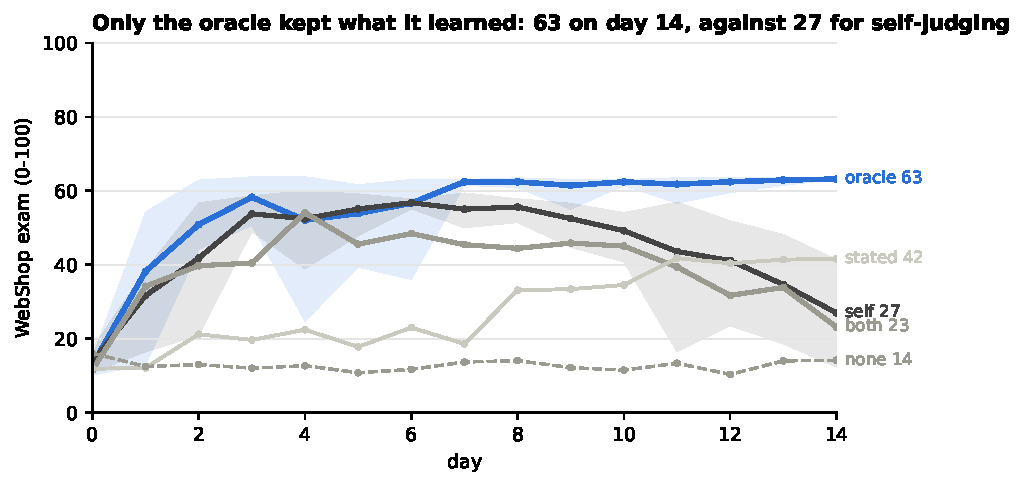
\includegraphics[width=1.0\linewidth]{figures/fig2_exp1_judges}
\caption{Experiment 1, 5 seeds per judge, daily exams; one self life crashed early and is left out}
\label{fig:2}
\end{figure}

On day 14 the \emph{oracle} averaged 63.2 $\pm$ 0.2 (mean $\pm$ standard deviation over seeds), \emph{self} 27.0 $\pm$ 11.9, \emph{both} 23.1 $\pm$ 17.0, \emph{stated verdict} 41.6 $\pm$ 23.1 and \emph{none} 14.2 $\pm$ 2.2. The \emph{stated verdict} learned from only 0-7 lessons per life, none of them a failure; three of its lives reached 54-61 and two stayed at 14-19. The \emph{oracle} beat \emph{self} and \emph{both} clearly (Welch t-test, p = 0.009 and 0.006); with 4-5 seeds, self-judging did not end reliably above no learning at all (p = 0.12).

Self-judging learned as fast as the \emph{oracle} at first and then lost most of it. By day 7 the \emph{self} and \emph{both} lives had reached 45-55; by day 14 every one of those nine lives had fallen below its own day-7 score, one to 0. The \emph{oracle} reached 62 by day 7 and stayed there. The \emph{stated verdict} rose slowly and unevenly (14-61 on day 14). One \emph{self} life crashed early and is left out. A 6-day pilot showed the same shape: the \emph{self} life rose from 13 to 34 by day 1 and fell to 9 by day 6.

\textbf{Does the decline pass with time?} We let the \emph{both} creature, the self-judge that also hears the user and the one that learned fastest early on, live for a year: 365 days, 5 seeds, beside one \emph{oracle} life. WebShop's practice tasks run out after about 227 days, so later days revisit old tasks.

\begin{figure}[htbp]
\centering
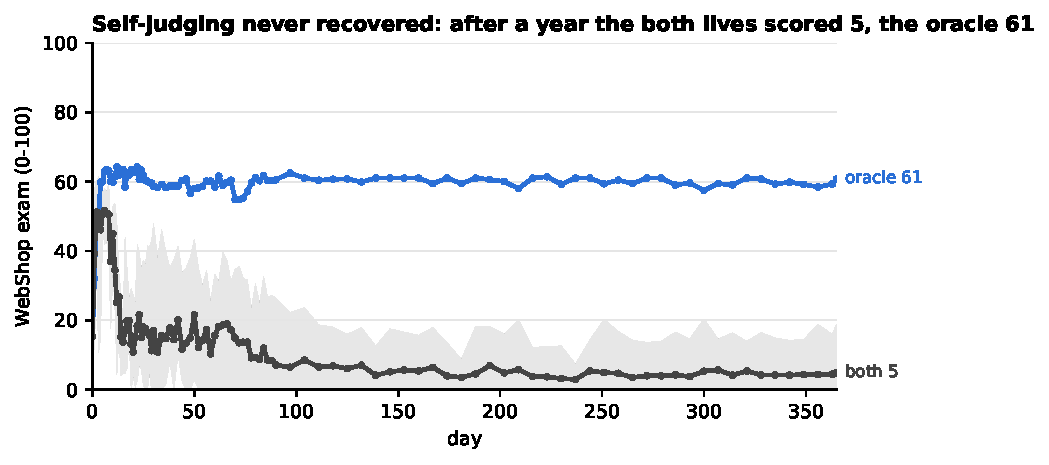
\includegraphics[width=1.0\linewidth]{figures/fig7_year_of_life}
\caption{Experiment 1, year of life: 5 both lives and 1 oracle life; exams daily to day 30, every 2 days to day 90, then weekly}
\label{fig:7}
\end{figure}

It never recovered. The \emph{both} lives peaked around day 6 (52, lives 42-58), were back at their starting level of 15 by day 14, and ended the year at 5 (0-19), three of the five at 0. The \emph{oracle} life rose from 15 to 64 by day 14 and stayed between 55 and 64 for the rest of the year (61 on day 365). These are separate lives from the 14-day \emph{both} condition above (23 on day 14, lives 0-46); the two ranges overlap. A first attempt at this run crashed when two nights ran out of GPU memory at once and was restarted from scratch.

\textbf{Is it the adapter?} If the adapter simply overwrote what it had learned, an adapter built to protect old learning might stop the decline. We gave the \emph{both} creature four designs, 5 seeds each for 14 days: one LoRA that keeps growing (as everywhere else), a LoRA whose learning rate halves every 4 days, a new rank-8 LoRA every 2 days with the older ones frozen, and the same with each new one smaller (rank 8 down to 1). All four peaked at 46-53 on day 7 and fell to 26-38 by day 14; the best of them still lost more than a quarter of its peak.

Neither time nor the adapter explains the decline. What the judge lets in does, and the rest of this section follows that thread.

\subsection{A separate, frozen judge: sense v2}

Experiment 2 gave the creature a judge it cannot change: the feedback sense (v2), a frozen Qwen3-0.6B with its own LoRA that reads the user's reaction to each attempt. It ran against the \emph{oracle} and \emph{both}, 5 seeds, 14 days, with the same user as Experiment 1.

{\def\LTcaptype{none} % do not increment counter
\begin{longtable}[]{@{}llll@{}}
\toprule\noalign{}
Judge & Day 0 & Day 7 & Day 14 \\
\midrule\noalign{}
\endhead
\bottomrule\noalign{}
\endlastfoot
\emph{oracle} & 11 & 62 (61-63) & 62 (61-63) \\
\emph{sense v2} & 13 & 19 (7-43) & 40 (6-59) \\
\emph{both} & 13 & 47 (36-57) & 16 (3-32) \\
\end{longtable}
}

\emph{Sense v2} learned more slowly but did not fall back. It also learned from very little: 0-7 lessons per life in 14 days, against 247-274 for the \emph{oracle}. By day 14, four of its five lives stood at 34-59 and were still rising, while every \emph{both} life had fallen from its day-7 peak. On day 14 \emph{sense v2} (39.7 $\pm$ 21.3) was ahead of \emph{both} (16.1 $\pm$ 11.1) and behind the \emph{oracle} (62.0 $\pm$ 1.0). With 5 seeds and one \emph{sense v2} life at 6, the t-test finds neither gap significant (p = 0.07 and 0.08); a rank test, less swayed by that one life, puts the gap to the \emph{oracle} at p = 0.01 (Appendix B). Sense v2's own accuracy stayed fixed, as intended: on 300 recorded reactions it read 82.6\% correctly on day 0 and 82.8\% on day 14. A variant that read the sense through the creature's learning brain was planned, but its lives scored 0 from day 0 because of a setup fault and were stopped; it is not reported.

\subsection{Realistic users break sense v2}

Experiment 3 replaced the user with one that reacts as people do. Its behaviour is drawn from a mix tied to the outcome and a persona, and worded by Gemini: clear thanks, complaints, but also polite give-ups, vague replies and moving on without a word. \emph{Oracle}, \emph{both} and \emph{sense v2}, 5 seeds, 14 days.

The \emph{sense v2} lives split in two. Two reached 55 and 57 by day 14, close to the \emph{oracle}'s 62. The other three fell to 0-3 on day 1 and never recovered. Each had learned on night 1 from one to three polite give-ups that sense v2 had read as success (Example 1 below); 96-100\% of everything those three lives learned were failed attempts. The \emph{both} lives rose to 48 by day 3 and fell to 15 (2-36). On day 14 the \emph{sense v2} lives averaged 22.5 $\pm$ 30.8 against the \emph{oracle}'s 62.0 $\pm$ 1.1 (Welch t-test p = 0.045, Mann-Whitney p = 0.01); the spread is the split itself.

\textbf{Example 1: a give-up sense v2 took for success (Experiment 3, night 1).} The shopper asked for men's loafers in size 6.5 under \$60. The creature bought nothing (reward 0). The user ended:

\begin{quote}
``That's perfectly fine, thank you so much for trying to help me! I think I'll just leave it for now and head out.''
\end{quote}

Sense v2 scored this reaction 100, the top score, with confidence 0.92, and the attempt became a lesson. All five practice attempts that became bad lessons on night 1 in the three collapsed lives look like this: warm thanks for the effort, then the user leaves.

Changing sleep did not remove the cause. When each lesson counted once, however many steps it took, and the creature slept only after 5 lessons, fewer lives collapsed, but 2 of 5 still ended at 0-3. The fault was in the judge, not the sleep.

\subsection{Waiting for a clear verdict: sense v3}

Experiment 4 used sense v3 (Section 3), our fullest attempt at discernment. It first asks whether the reaction is a clear verdict on the result; thanks for the effort, sarcasm, hedging, silence or moving on count as no verdict, and nothing is learned from them. Only a clear verdict is then scored. Same user and conditions as Experiment 3.

On 2,622 recorded reactions from Experiment 3, sense v3 read 1.2\% of reactions that were neither praise nor acceptance as a yes, against 5.0\% for v2, and read 1.0\% of give-ups and polite complaints as success, against 15.8\% (Fig.~\ref{fig:3}; Fisher exact test, p \textless{} 0.001). The price was a stricter reading of real approval: it took 59\% of plain acceptances as a yes, against 70\% for v2. In the lives, four of five \emph{sense v3} lives stood at 53-60 on day 14, against the \emph{oracle}'s 63 (62-63). Averaged over all five lives \emph{sense v3} (45.1 $\pm$ 25.3) was not reliably below the \emph{oracle} by a t-test (62.8 $\pm$ 0.6; p = 0.19), because the one collapsed life dominates the spread; by a rank test it was (p = 0.01), since every \emph{sense v3} life scored below every \emph{oracle} life. The fifth fell to 0 after learning from a single give-up on night 1. The \emph{both} lives peaked at 53 on day 7 and fell to 19 by day 14, as before.

\begin{figure}[htbp]
\centering
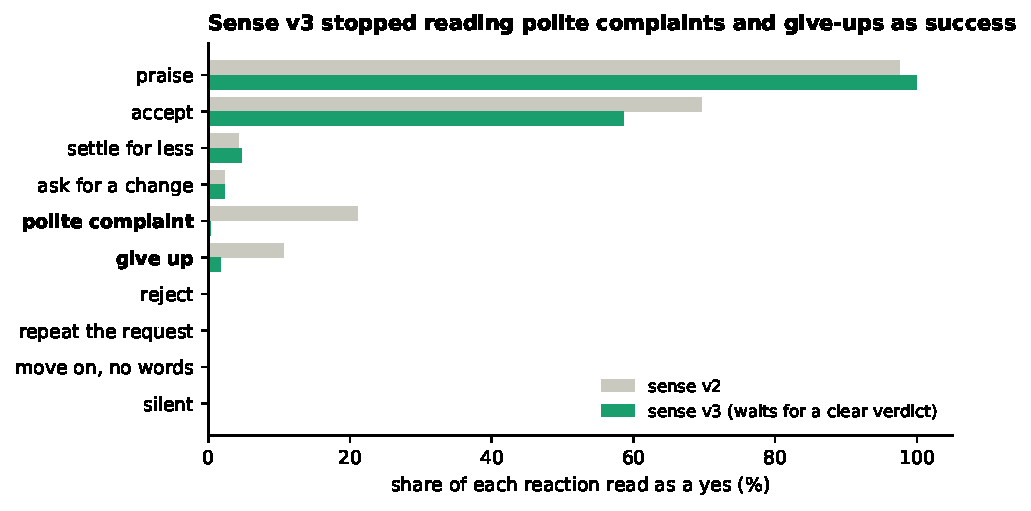
\includegraphics[width=1.0\linewidth]{figures/fig3_sense_v2_v3}
\caption{Sense live test: up to 300 recorded reactions per behaviour from the Experiment 3 lives (2,622 in all), read by both versions of the sense}
\label{fig:3}
\end{figure}

\subsection{Clean but scarce lessons fade: sense v3 over 60 days}

Every life of Experiment 4 was extended to 60 days.

\begin{figure}[htbp]
\centering
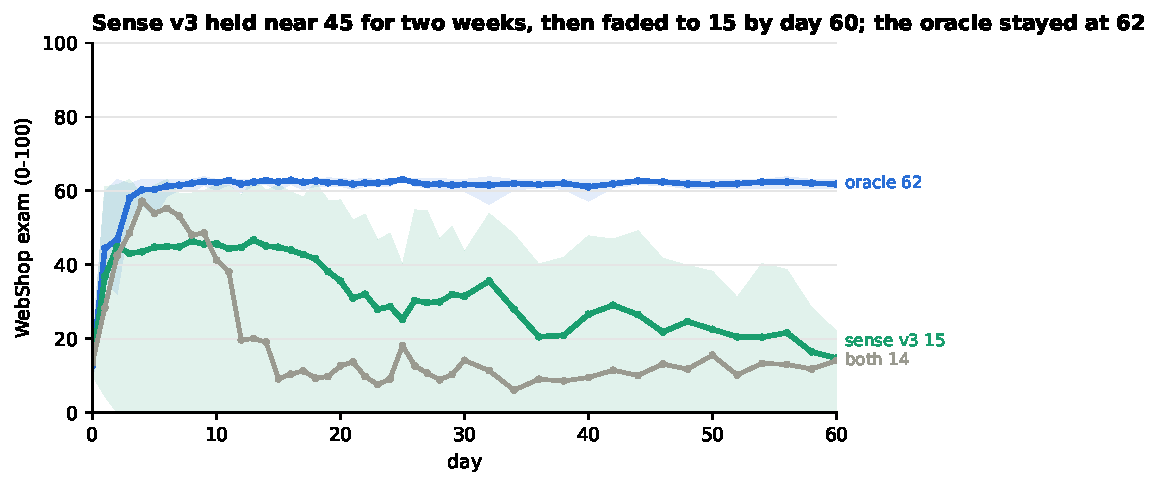
\includegraphics[width=1.0\linewidth]{figures/fig4_sense_v3_60_days}
\caption{Experiment 4, 5 seeds per judge, 60 days; exams daily to day 30, then every 2 days}
\label{fig:4}
\end{figure}

Life by life, the four \emph{sense v3} lives that did not collapse stood at 53-60 on day 14, 36-44 on day 30 and 9-22 on day 60; the fifth stayed at 0 throughout. On day 60 the \emph{oracle} (61.8 $\pm$ 0.9) was far above \emph{sense v3} (14.7 $\pm$ 9.7; Welch t-test p \textless{} 0.001).

The four \emph{sense v3} lives declined steadily after day 14, although what they learned stayed clean. They took in about 2 lessons a day (1.6-2.4), against the \emph{oracle}'s 20-21, and learned from only 10-13\% of their own good attempts, because a clear yes was rare. Over the 60 days only 2-10\% of their lessons were failed attempts. The collapsed life stayed at 0 for all 60 days, replaying its bad lessons (Fig.~\ref{fig:4}). Why they faded is open. Scarcity alone is not an obvious answer, since in Experiment 2 lives with even fewer lessons kept rising to day 14; an \emph{oracle} limited to 2 lessons a day would settle it.

\subsection{What every life has in common}

Across the WebShop experiments (1-4, including the adapter designs of 5.1), what decided a life was the share of its lessons that were failed attempts, not the number of lessons or the kind of judge.

\begin{figure}[htbp]
\centering
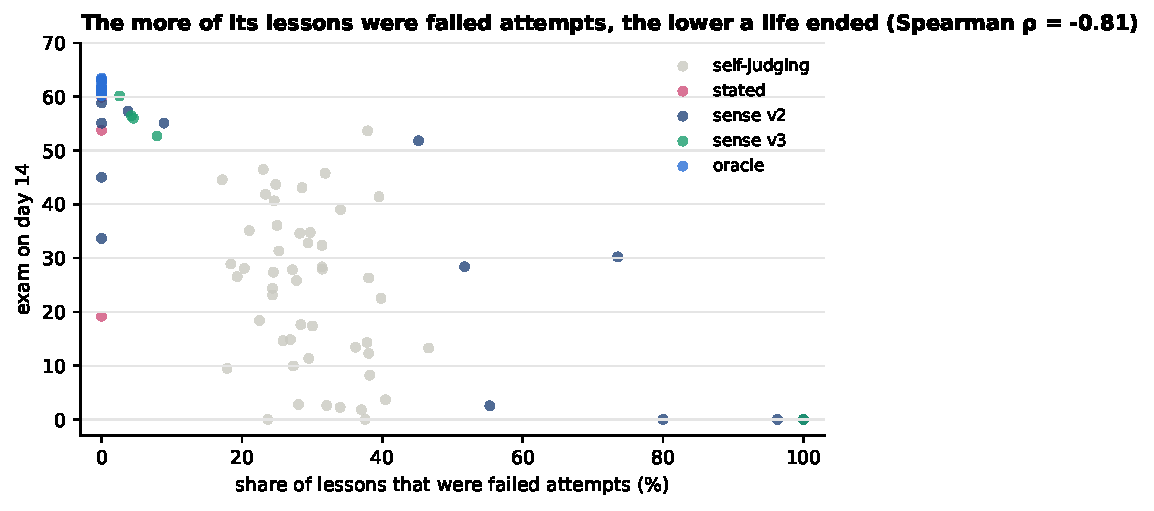
\includegraphics[width=1.0\linewidth]{figures/fig6_failed_lessons}
\caption{All 14-day WebShop lives in Experiments 1-4, including the adapter designs of 5.1, that learned at least once (97 of 104); lessons counted to day 14; Exp 3b = the sleep variant of Experiment 3}
\label{fig:6}
\end{figure}

Across 97 lives, the share of failed attempts among a life's lessons in its first 14 days predicted its day-14 exam closely (Spearman $\rho$ = -0.81, p \textless{} 0.001). The \emph{oracle} lives, all at 0\% failures and about 63, do not drive this alone: among the 72 lives not judged by the \emph{oracle}, $\rho$ = -0.61 (p \textless{} 0.001). Every \emph{oracle} life learned only from successes and ended at 60-63. Self-judging lives let in 17-47\% failures and ended anywhere from 0 to 54. The sense lives, v2 and v3 together, split cleanly: the ten that let in under 10\% failures ended at 34-60; the nine that let in 45\% or more ended at 0-52, six of them at 0-3.

The number of lessons mattered less than we expected. In Experiment 2 the \emph{sense v2} lives learned from only 0-7 lessons in 14 days and still reached 34-59; in Experiment 1, the \emph{stated verdict} learned from 0-7, none of them failures, and reached up to 61. A few correct lessons are enough to teach the shop's basic routine, and a few wrong ones are enough to undo it.

This explains why a single bad night can end a sense life. A sense life learned from only 0-6 lessons on night 1, so one failed attempt could be most of its first night's training. Of the 20 sense lives in Experiments 2-4 (v2 in Experiments 2 and 3, v3 in Experiment 4), seven learned from a failed attempt on night 1, and six of those seven ended at 0-3 (Fisher exact test, p \textless{} 0.001). Of the thirteen without one, none ended below 28, except one that never learned anything at all (6).
